%!TEX root = ../paper.tex
\chapter{DVB-T系统概述}
	\section{DVB-T系统结构与原理}
	\label{sec:dvbt_summary}
		\par 地面数字视频广播(Digital Video Broadcasting-Terrestrial,DVB-T),是欧洲广播联盟在1997年发布的数字地面电视视频广播传输,最早于1998年在英国实行广播\ucite{wiki:DVB-T}。
		\par 由于地面电视的特殊环境,DVB-T系统选定了码分正交频分复用(COFDM)的信道调制技术,并使用RS编码、符号交织、比特交织等技术,达到传输可靠性和频谱利用效率的相对平衡。DVB-T系统提供了两种子载波数量(2K模式和8K模式),3种调制方式(QPSK,16QAM和64QAM),4种保护间隔(1/4,1/8,1/6和1/32),系统支持目前模拟电视系统的6MHz,7MHz和8MHz带宽,还支持等级调制\ucite{what_is_dvb_t}。
		\par 图\ref{fig:dvbt_tx}描述了DVB-T发射端系统。
		\begin{figure}[htp]
			\centering
			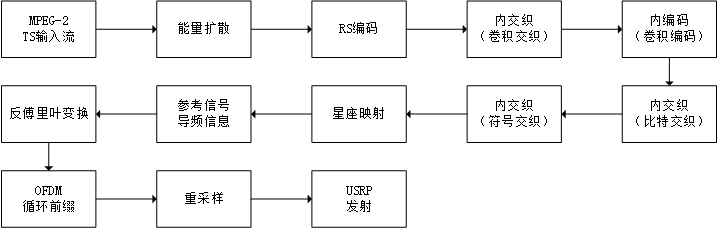
\includegraphics[width=13cm]{figures/dvbt_tx.png}
			\caption{DVB-T发射端}
			\label{fig:dvbt_tx}
		\end{figure}
		\par 图\ref{fig:dvbt_rx}描述了DVB-T接收端系统。
		\begin{figure}[htp]
			\centering
			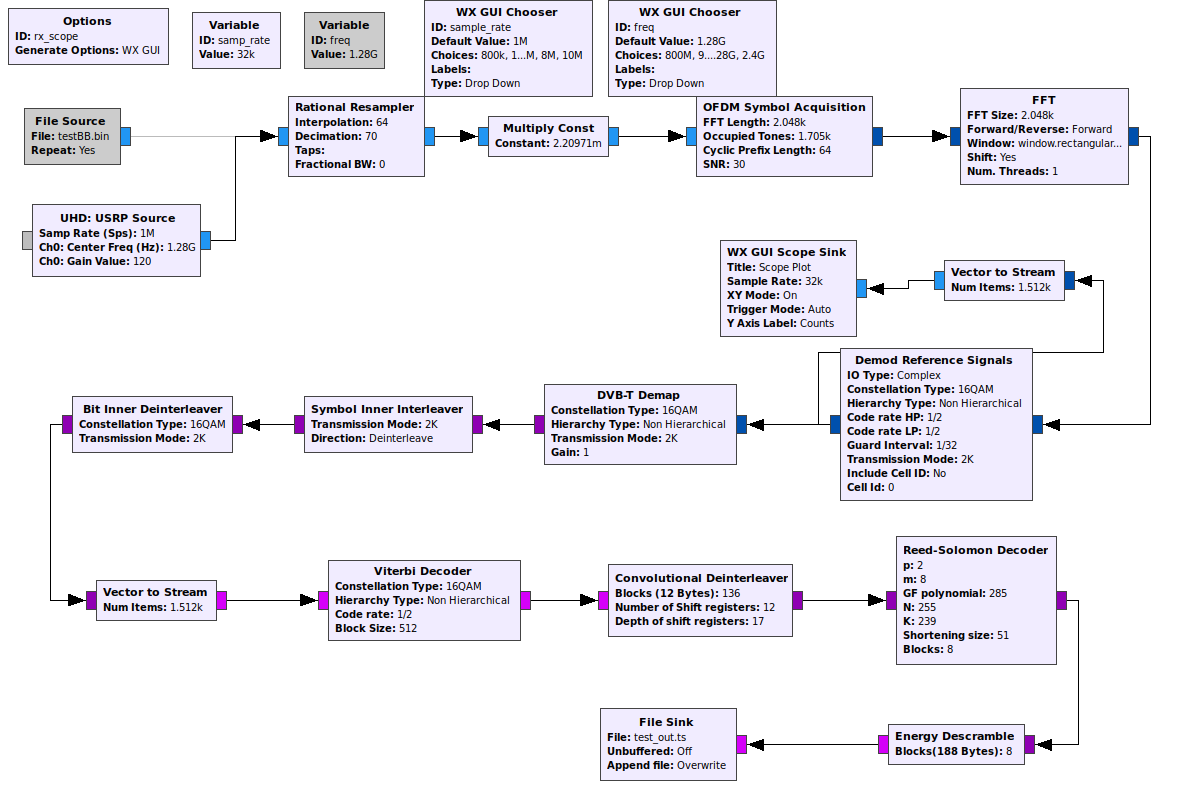
\includegraphics[width=13cm]{figures/dvbt_rx.png}
			\caption{DVB-T接收端}
			\label{fig:dvbt_rx}
		\end{figure}
		\par DVB-T系统中可以调节的参数见表\ref{table:params_of_dvbt}。
		\begin{table}[!htbp]
			\centering
			\caption{DVB-T供调节参数}
			\begin{tabular}{|l|p{0.6\columnwidth}|}
				\hline\hline
				内纠错码率(FEC) & 1/2 , 2/3 , 3/4 , 5/6 , 7/8                            \\
				\hline
				子载波调制方式    & QPSK , 16QAM , 64QAM                                   \\
				\hline
				保护间隔             & 1/4 , 1/8 , 1/16 , 1/32                                \\
				\hline
				等级调制参数       & $\alpha$=1(等级) , $\alpha$=2 , 4(非等级) \\
				\hline
				载波数量             & 2k : 1705 , 8k : 6817                                  \\
				\hline\hline
			\end{tabular}
			\label{table:params_of_dvbt}
		\end{table}
		\endinput